%  Robotics Text  by Jacob Rosen and Blake Hannaford
% (c) 2007  Jacob Rosen and Blake Hannaford
%

\chapter{Kinematic Redundancy}\label{KinematicRedundancyChapter}

\section{Problem Statement and Learning Objectives}
% Problem Statement and Learning Objectives for Chapter 13


\section{The Pseudoinverse}


The basic problem is solving the velocity equation
\begin{equation}
\dot{x}=J\dot{\theta}
\end{equation}
when the diminsions of $\dot{x}$ and $\dot{\theta}$ are not the same.
Let us call the dimensionality of the task space $n$ and the number of
joints, $m$.  The Jacobian matrix, $J$, has dimensions $n\times m$ and
we cannot invert a non-square matrix.  Let's consider three cases:
\begin{enumerate}
   \item $m > n$ (\# joints $>$ \# task freedoms) \\
   $\dot{\theta} $ is ``bigger'' than $\dot{x}$.  There are thus many
possible solutions (many joint velocities for the same end-effector
velocity).

    \item $m = n$ \\

    If $\mathrm{rank}(J) = m = n$,  $\dot{\theta} = J^{-1} \dot{x}$.

    \item $m < n$ \\
     $\dot{\theta} $ is ``smaller'' than $\dot{x}$.  There is no
solution.  However, we might be interested in a joint velocity vector
which is closest to a solution.

\end{enumerate}

\paragraph{Moore-Penrose Pseudo-Inverse}

Let's look at how to invert a non-square matrix by first looking at some
properties of a square inverse:

If we choose a square matrix $A$, which is full rank, and compute its
inverse: $X = A^{-1}$, then we have
\begin{equation}\label{MPC0}
X A = I
\end{equation}
There are also four similar properties (Penrose conditions) which are
true:
\begin{equation} \label{MPC1}
AXA = A
\end{equation}
\begin{equation}\label{MPC2}
XAX = X
\end{equation}
\begin{equation}\label{MPC3}
(AX)^{T} = AX
\end{equation}
\begin{equation}\label{MPC4}
(XA)^{T} = XA
\end{equation}

When $A$ is non-square, we cannot satisfy \ref{MPC0}, but various
schemes can give us a matrix which satisfies one or more of
\ref{MPC1} --- \ref{MPC4}.

The matrix $A^{+}$, called the Moore-Penrose inverse or also the
{\it pseudoinverse}, satisfies \ref{MPC1} --- \ref{MPC4}.
In addition, it satisfies two more properties:
\begin{equation} \label{MPC5}
(A^{+})^{+} = A
\end{equation}
\begin{equation}\label{MPC6}
(A^T)^{+} = (A^{+})^T
\end{equation}


  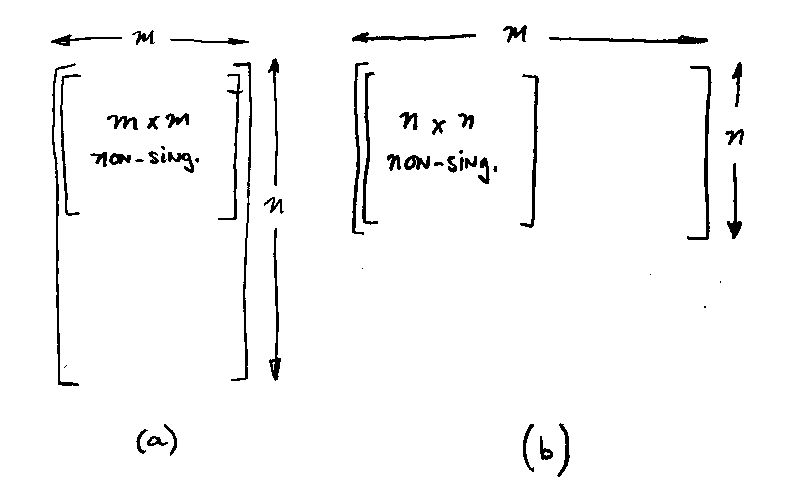
\includegraphics[width=5.5in]{figs13/00096.eps}

\paragraph{Computation of $A^+$}

The definition of $A^{+}$ depends on the structure of $A \br^{n \times m}$ as follows:
\begin{enumerate}

    \item if $\mathrm{rank}(A) = m$ \\
    $A^{+} = A^T(AA^T)^{-1}$ \\
    (see illustration (a)).

    \item if $\mathrm{rank}(A) = n$ \\
        $A^{+} = (AA^T)^{-1}A^T$ \\
    (see illustration (b)).

    \item otherwise, if the SVD of $A$ is  \\
\[
A = U \Sigma V^T
\]
    and $\mathrm{rank}(A) = r$, then

\[
A^{+} = V \Sigma^{+} U^T
\]
where
\[
\Sigma^+ =  \left [
\begin{array}{cccccc}
\sigma_1^{-1}          & 0 & 0 & 0 & | & 0\\
0 & \sigma_2^{-1}          & 0 & 0 & | & 0\\
0 & 0 & \dots                  & 0 & | & 0\\
0 & 0 & 0 & \sigma_r^{-1}          & | & 0\\
- & - & - & - & -                      & 0\\
0 & 0 & 0 & 0 & 0                      & 0\\
\end{array}
\right ]
\]

\end{enumerate}



\paragraph{Solving Equations}

Let's apply this to solve equations.  We will start with
\begin{equation}
y = As
\end{equation}
where $y \br^n$ and $s \br^m$.   Let's consider the case, $m>n$.  It turns
out, the pseudo inverse allows us to write:
\begin{equation}\label{MPSoln}
s = A^{+}y + (I-A^{+}A)z
\end{equation}
where $z$ is an arbitrary vector which selects among multiple
solutions. One possible value for $z$ is 0 which gives.
\[
s_0 = A^{+}y
\]

It turns out $s_0$ has the smallest Euclidian norm of any solution. This
is true because the two terms:
\[
     A^{+}y \quad \mathrm{and} \quad (I-A^{+}A)z
\]
are orthogonal to each other.

Exercise: Recall that for any orthogonal vectors $q, v$, $q^Tv =0$.
Use this to show the terms above are orthogonal.



\section{Accomplishing Additional Tasks (Task Decomposition)}



\paragraph{Solving inverse velocity problem I: Additional Task}

Now we can return to the problem
\[
\dot{x} = J \dot{\theta}
\]
for the kinematically redundant manipulator.  Using eqn. \ref{MPSoln},
we have
\begin{equation}\label{KRSoln}
\dot{\theta} = J^{+}\dot{x} + (I-J^{+}J)\dot{z}
\end{equation}
where $\dot{z} $ is an arbitrary vector to select among solutions.

The columns of $(I-J^{+}J)$ define the {\it null space} of $J$, i.e. a
subspace of the joint space in which joint motion causes zero end
effector velocity.

{\bf Definition: }  The null space of a matrix $A$, is the set of all
non-zero $x$ such that
\[
Ax = 0
\]

Let's apply this to eqn \ref{KRSoln}:

Let $\hat{\dot{\theta}} = (I-J^{+}J)\dot{z}$.   Then
\[
\hat{\dot{x}} = J\hat{\dot{\theta}}
\]
\[
 =  J (I-J^{+}J)\dot{z}
\]
\[
 =  (J - JJ^{+}J) \dot{z}
\]
\[
 = 0
\]

by the first Penrose condition (eqn. \ref{MPC1}).
So the arbitrary vector $\dot{z}$ causes joint motion, but causes
no end effector motion. We call this type of motion,

``Self Motion"

``Null-space motion"

The matrix $  (I-J^{+}J)$ projects $\dot{z}$ into the null-space of the
manipulator.  The dimensionality of the null-space is
\[
\mathrm{rank}(I-J^{+}J)
\]
which is $m - n$ or the number of joints, minus the number of task DOF.

\paragraph{Example: 7 DOF Robotics Research Arm}

We will use a specific example to illustrate how the vector  $\dot{z}$
can be used to satisfy an additional task.

$m=7$, $n=6$

\begin{tabular}{cc}

 \scalebox{1.5}{
   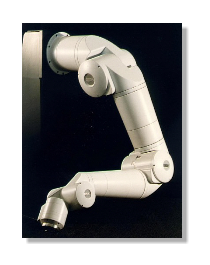
\includegraphics{figs13/00084.eps}
   }

& 

 \scalebox{0.4}{
   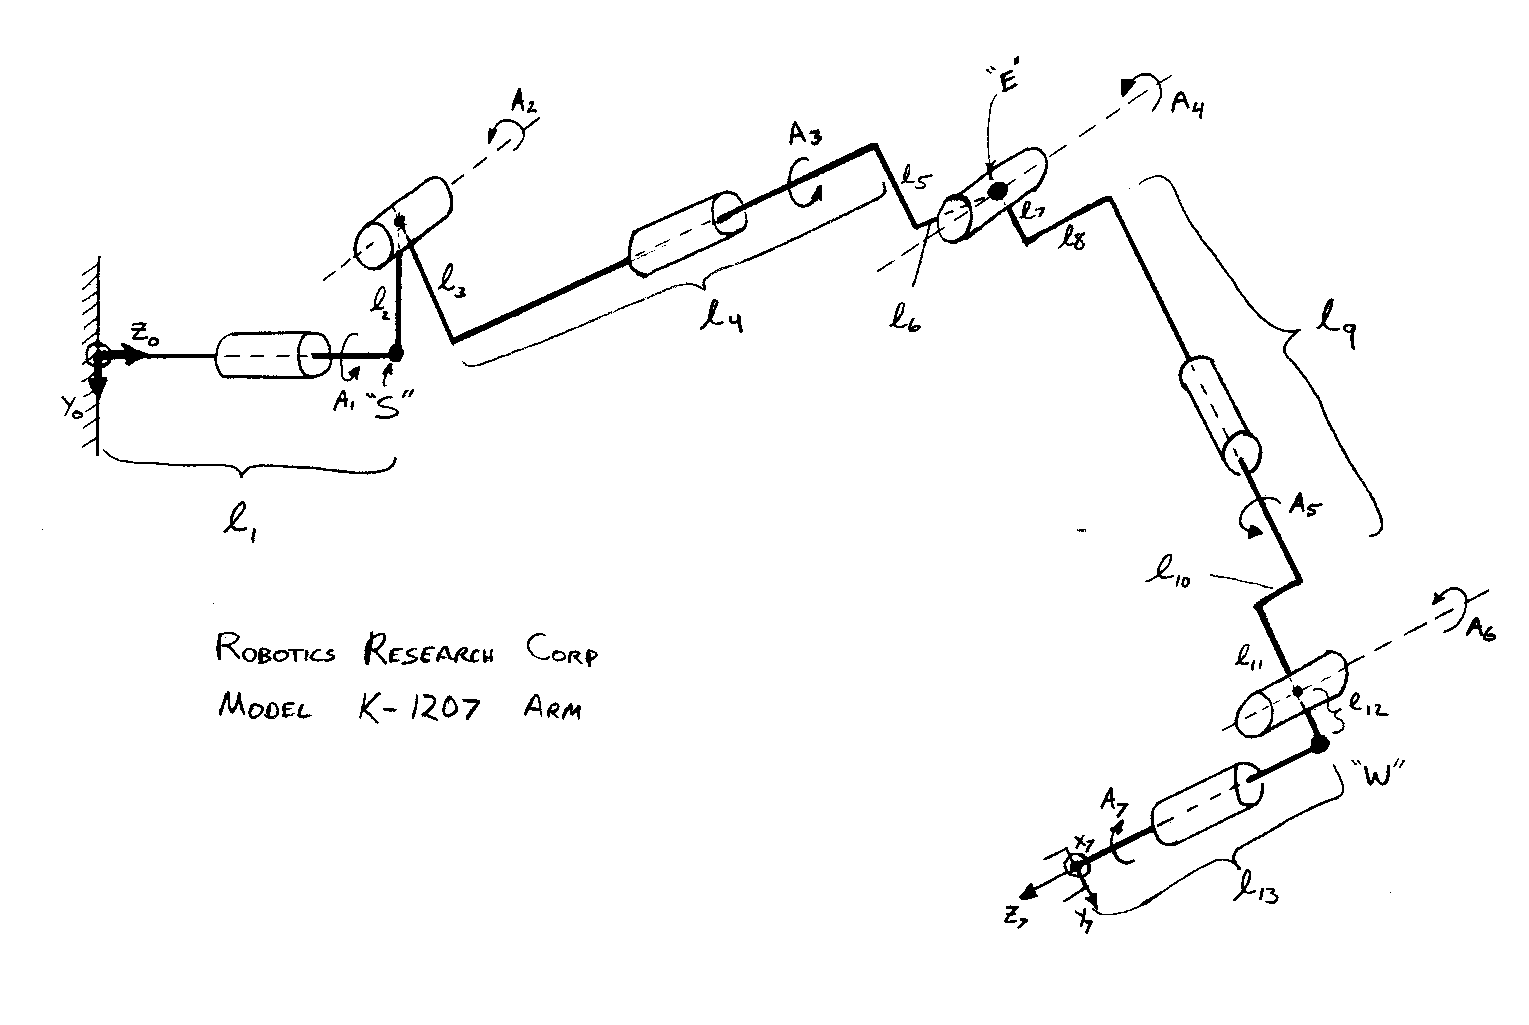
\includegraphics{figs13/00085.eps}
  }
\end{tabular}

The Robotics Research Arm is a 7-DoF arm (figure).   It   has one
DOF left over after the 6 DOF end effector positioning task is
satisfied.  The joint offsets ($l_2, l_3, l_5, l_8, 1_{10}, l_{12}$)
make the kinematic equations for this arm very complex.

We will assume that the inverse kinematics of the arm have
been solved, but we note that the same issue exists with regular inverse
kinematics as with the Jacobian inversion.  There are more unknown joint
variables than equations.

When this arm performs self-motion, it's elbow rotates in a circle
around an imaginary line connecting the shoulder and wrist.  This is especially 
easy to see if we draw a simplified version of this manipulator as follows:

 \scalebox{1.0}{
   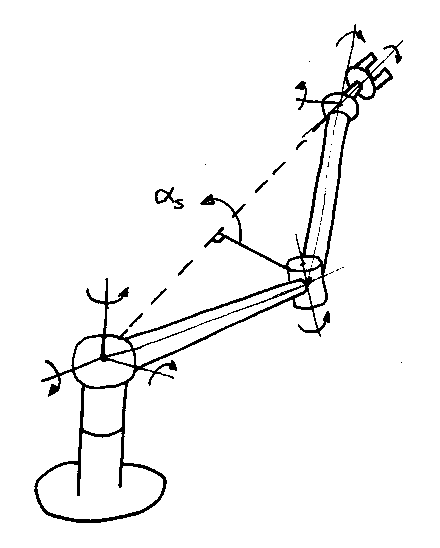
\includegraphics{figs13/00100.eps}
   }

Now these offsets have been removed and we can more easily imagine the elbow
being able to swing around in a circle without moving the end effector's position
or orientation.
We will add one more ``DOF'' to the {\em task} by specifing the angle of a
ray between this imaginary line and the elbow.  We will call this angle
$\alpha_s$.

Without solving for this angle, we will assume that there is some
function which specifies
\[
\alpha_s = f(\theta)
\]
We also assume that this can be differentiated:
\[
\dot{\alpha_s} = J_s(\theta) \dot{\theta}
\]
where $J_s$ is an $m \times 1$ vector:
\[
J_s = \left [
\begin{array}{cccc}
\frac{\pd \alpha_s}{\pd \theta_1}, &
\frac{\pd \alpha_s}{\pd \theta_2}, &
\dots &
\frac{\pd \alpha_s}{\pd \theta_m}
\end{array}
\right ]
\]

Now we can specify an additional   task,
\[
\dot{\alpha_s} = \dot{\alpha}_d
\]
in addition to the usual
\[
\dot{x} = \dot{x}_d
\]
Now we can make use of the additional DOF to make use of the extra
flexibility of this arm.

First, we recall the solution for the redundant arm (eqn \ref{KRSoln}).

\[
\dot{\theta} = J^{+}\dot{x} + (I-J^{+}J)\dot{z}
\]

The basic strategy will be to assume that tasks can be satisfied by
some $\dot{z}$ and then solve  eqn \ref{KRSoln} for  $\dot{z}$.

let
\[
\dot{x} = \dot{x}_d,  \dot{\alpha_s} = \dot{\alpha}_d
\]
\[
\dot{\alpha}_d = J_s ( J^{+}\dot{x}_d + (I-J^{+}J)\dot{z})
\]
\[
\dot{\alpha}_d = J_s J^{+}\dot{x}_d + J_s(I-J^{+}J)\dot{z}
\]

\[
\dot{\alpha}_d - J_s J^{+}\dot{x}_d = J_s(I-J^{+}J)\dot{z}
\]
Now let
\[
\tilde{J}_s = J_s(I-J^{+}J)
\]

Using eqn \ref{MPSoln},

\[
\dot{z} = \tilde{J}_s^{+}(\dot{\alpha}_d - J_s J^{+}\dot{x}_d) +
(I-\tilde{J}_s^{+}\tilde{J}_s)\dot{y}
\]

Let's look at what we have.   Now, assuming that we have chosen
an end-effector task, $\dot{x}$, and an elbow-angle task
$\dot{\alpha}_s$, then we now have a way to get $\dot{z}$.

\[
(I-\tilde{J}_s^{+}\tilde{J}_s)
\]
describes the null-space of $\tilde{J}_s$ and the size of this null
space tells us how many DOF are left {\it after} the elbow-angle task is 
complete.
If our subtask (i.e.  $\dot{\alpha_s} = \dot{\alpha}_d$) uses
up all the remaining freedoms in the arm (which it does in this case),
then   $\mathrm{rank}((I-\tilde{J}_s^{+}\tilde{J}_s))=0$.

Now we can plug $\dot{z}$
back into the original solution (eqn. \ref{KRSoln}) to get
\[
\dot{\theta}_d = J^{+}\dot{x}_d +
(I-J^{+}J)\tilde{J}_s^{+}(\dot{\alpha}_d-J_sJ^{+}\dot{x}_d)
\]
Yoshikawa (cf page 247 \& eqn 7.9)
shows that
\[
(I-J^{+}J)\tilde{J}_s^{+} =  \tilde{J}_s^{+}
\]
so a simpler form of the solution is:
\[
\dot{\theta}_d = J^{+}\dot{x}_d +
\tilde{J}_s^{+}(\dot{\alpha}_d-J_sJ^{+}\dot{x}_d)
\]

For the RRC arm, we have introduced an additional task
($\dot{\alpha_s} = \dot{\alpha}_d$) and used up all the mechanism's
freedom.   Sometimes this may not be clear.  In general, we can evaluate
\[
(I-\tilde{J}_s^{+}\tilde{J}_s)
\]
If it is not equal to zero, the manipulator has additional capability to
do another task.




\subsection{Rank M-1}
\subsection{More Redundancy}

\section{Optimization using Redundant Degrees of Freedom}



\paragraph{Solving inverse velocity problem II: Optimization of Pose}

\paragraph{Introduction}
As an alternative to using an explicit additional task, we might want to use the
kinematic redundancy to optimize some performance measure such as
manipulability.  Let's call the performance measure:

\[
p = V(\theta)
\]


Define $\dot{z}_d$ as
\[
\dot{z}_d = K_p \grad p = K_p
\left [
\begin{array}{cccc}
\frac{\pd p}{\pd \theta_1}, &
\frac{\pd p}{\pd \theta_2}, &
\dots &
\frac{\pd p}{\pd \theta_m}
\end{array}
\right ]^T
\]

Now we are performing a sort-of mechanical gradient ascent and we can
see the two  approaches are the same.   This gives us
\begin{equation}\label{GradSoln}
\dot{\theta}_d = J^{+}\dot{x} + (I-J^{+}J)K_p\grad p
\end{equation}

\paragraph{Improvement of Performance}


Let's try to show that with $\dot{z}$ defined as above,
the null space motion will not not decrease $p$\footnote{
See {\it Characterization of Optimal Solutions in Kinematic Resolutions of
Redundancy}, by J. Park, W.K. Chung, Y. Youm,
IEEE Trans. Robotics and Automation, v 12., no 3, pp. 471-478, June 1996.}.

\begin{equation}\label{GradP}
\frac{dp}{dt} =  \frac{\pd p}{\pd \theta_1}\frac{\pd \theta_1}{\pd t} +
\frac{\pd p}{\pd \theta_2}\frac{\pd \theta_2}{\pd t}  +
\dots +
\frac{\pd p}{\pd \theta_m}\frac{\pd \theta_m}{\pd t}
\end{equation}

\begin{equation}
\renewcommand*{\arraystretch}{1.5}
= \left [
\begin{array}{cccc}
\frac{\pd p}{\pd \theta_1}, &
\frac{\pd p}{\pd \theta_2}, &
\dots &
\frac{\pd p}{\pd \theta_m}
\end{array}
\right ]
\left [
\begin{array}{c}
\frac{\pd \theta_1}{\pd t} \\
\frac{\pd \theta_2}{\pd t} \\
\dots \\
\frac{\pd \theta_m}{\pd t} \\
\end{array}
\right]
\end{equation}

\[
= \grad p^T \dot{\theta}
\]
Using eqns  \ref{GradSoln} and \ref{GradP},
\[
\frac{dp}{dt} = (\grad p)^T (J^{+}\dot{x} + (I-J^{+}J)K_P \grad p)
\]

\begin{equation}\label{Psoln}
\dot{p} =(\grad p)^T J^{+}\dot{x}  +(\grad p)^T (I-J^{+}J)K_P \grad p
\end{equation}

The two terms in eqn \ref{Psoln} represent the main task of end effector
motion and the subsidiary task of kinematic optimization respectively.
The first term may {\it reduce or increase} $p$ because it is not related
to the gradient of $p$.
The second term always moves the arm in a way that does not decrease $p$.
Note that these two terms may ``fight'' each other.

\paragraph{Examples of performance functions}

\begin{enumerate}
\item Manipulability --- Drive the null space motion in such a was that manipulability
(of the end effector) is maximized.

\item Distance from singular points.  Use a performance measure such as kinematic
conditioning index (ratio of smallest to largest singular value) as performance
measure.

\item Distance from joint limits.  This one is really important for real-world
implementations.  Define a performance function, $P_{JL_n}$,
which is zero at joint limits and maximized in between.

Example:
\scalebox{1.0}{
  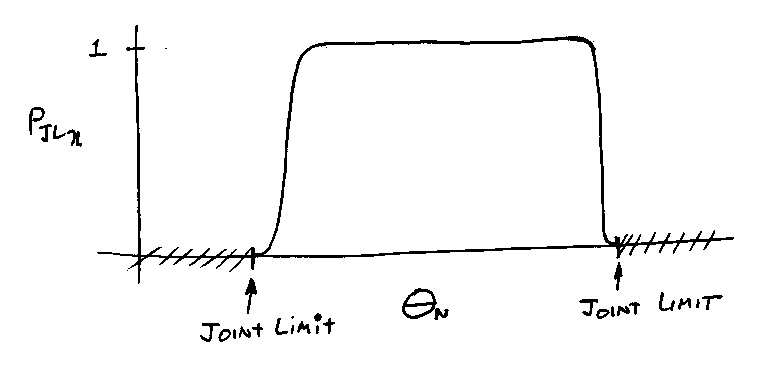
\includegraphics{figs13/00097.eps}
  }

\item Height of elbow off the ground ($Z_{elbow}$, the Z component of elbow position.)

\scalebox{1.0}{
  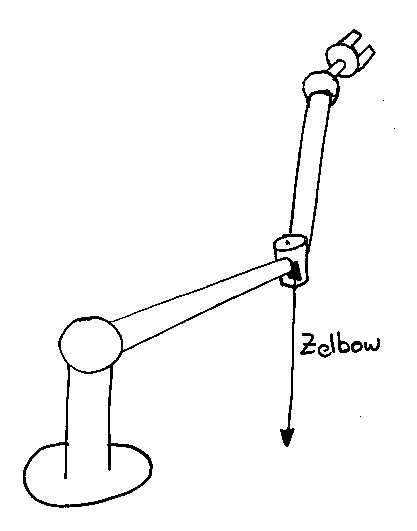
\includegraphics{figs13/00098.eps}
  }

\item ``Potential function energy'' ---  a virtual energy attached to the inverse
of distance between the robot and environmental obstacles.

\end{enumerate}


\section{Applications}
Obstacle Avoidance\\
Avoiding Singularities

\section{Joint Velocity - Computational Method}

\section{Hyperredundant Manipulators}
Brief look at snake robots.


\section{Summary of Notation}

% Summary of Notation for Chapter  13

